\section{Ejercicios}

Estimado estudiante, realizar los siguientes ejercicios de manera clara y ordenada.
Tener presente siempre justificar sus respuestas en los ejercicios que lo requieren.
Se tendrá una duración máxima de 50 minutos para resolver la prueba (2:30 minutos por ejercicio).

\begin{exercise}
    Relacione (utilizando líneas) los siguientes símbolos con su significado.
    \begin{align*}
        1.\ \ \Z &&\ && &\text{a. Los racionales.}\\
        2.\ \ \R &&\ && &\text{b. Los complejos.}\\
        3.\ \Q^' &&\ && &\text{c. Los naturales.}\\
        4.\ \ \N &&\ && &\text{d. Los reales.}\\
        5.\ \ \Q &&\ && &\text{e. Los irracionales.}\\
        6.\ \ \C &&\ && &\text{f. Los enteros.}
    \end{align*}
\end{exercise}

\begin{exercise}
    Ubique gráficamente los conjuntos de números en la siguiente figura.
    \begin{figure}[H]
        \centering
        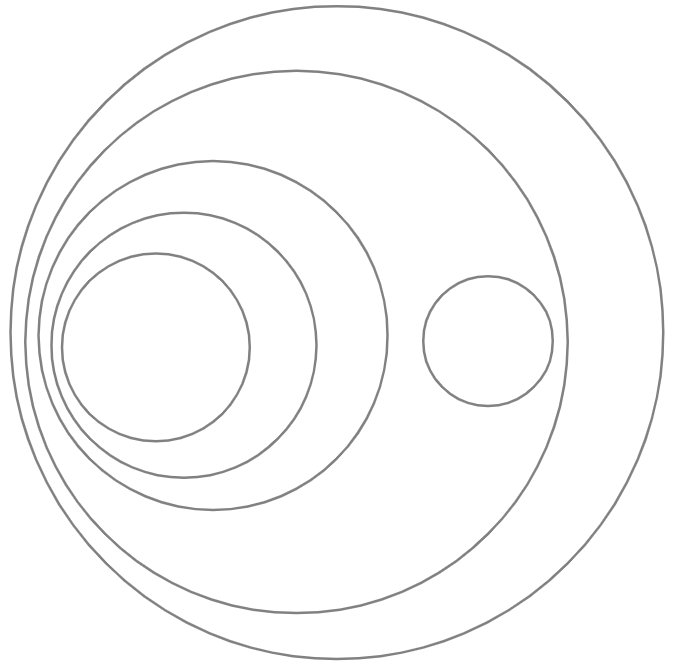
\includegraphics[width=10cm]{image/diagram}
        \label{fig:figure1}
    \end{figure}
\end{exercise}

\begin{exercise}
    Determinar la opción correcta sobre las siguientes proposiciones.
    \begin{tasks}[label=\Roman*.](4)
        \task $-5 \in \N$
        \task $0 \in \Z$
        \task $\frac{\sqrt{40}}{0} = 2 \in \Q$
        \task $\frac{\pi}{3.1416} \notin \Q^'$
    \end{tasks}
    \begin{tasks}(5)
        \task FVFV
        \task FVVV
        \task FVVF
        \task FVFF
        \task VVFF
    \end{tasks}
\end{exercise}
\\
\vspace{4.5cm}

\begin{exercise}
    Un profesor interroga a sus cinco estudiantes: \textit{¿Quién jodido se copió en la prueba?}, y ellos respondieron lo siguiente:
    \begin{multicols}{2}
        \textbf{Gerald:} Lo hizo Nahomi. \\
        \textbf{Brisa Marina:} Nahomi fue. \\
        \textbf{Fabiana:} Sharloth lo hizo. \\
        \textbf{Nahomi:} Yo no fui. \\
        \textbf{Sharloth:} Brisa Marina no se copió. \\
    \end{multicols}
    Si uno de ellos lo hizo y es compañero de Gerald, además solo uno dice la verdad, ¿quíen fue el que se copió?
\end{exercise}
\\
\vspace{6cm}

\begin{exercise}
    Si $a = 0.3$, encontrar el valor de $7a + 2$ y expresarlo en una fracción.
\end{exercise}
\\
\newpage

\begin{exercise}
    Escribir los elementos del conjunto $\{x\ |\ x^2 < 30,\ \text{con } x \ \text{par}\}$.
\end{exercise}
\\
\vspace{5cm}

\begin{exercise}
    Simplificar el siguiente producto
    \[
        \left(1 - \inverseOf{3}\right)\left(1 - \inverseOf{4}\right)\left(1 - \inverseOf{5}\right)\ldots\left(1 - \inverseOf{16}\right)
    \]
\end{exercise}
\\
\vspace{7.5cm}

\begin{exercise}
    Sabiendo que $(b \# a)^2 = a(a \# b)$ con $a # b > 0$.
    Hallar el valor de $20 \# 3$.
\end{exercise}
\\
\newpage

\begin{exercise}
    Se tiene 3 números consecutivos, el duplo del menor más el triple del mediano, más el cuádruple del mayor equivale a 74.
    Hallar el número menor.
\end{exercise}
\\
\vspace{5cm}

\begin{exercise}
    Sabiendo que $xy = 36$, $yz = 64$ y $zx = 9$.
    Encontrar el valor de $\dfrac{xyz}{4}$, sin calcular los valores de $x,y$ y $z$.
\end{exercise}
\\
\vspace{4cm}

\begin{exercise}
    Calcular el valor de $M = 7^2 - 6^2 + 2^4 + (0.2)^2 + \dfrac{24}{25} - \left(\inverseOfD{3}\right)^{-1}$
\end{exercise}
\\
\vspace{4cm}

\begin{exercise}
    Calcular el valor de $M = \left(\inverseOfD{3}\right)^{-3} + \left(\inverseOfD{4}\right)^{-2} + \left(-\inverseOfD{7}\right)^{-1} - \left(\inverseOfD{6}\right)^{-2} + 1$.
\end{exercise}
\\
\newpage

\begin{exercise}
    Hallar el valor de $m + n$ si $\left(x^{2n + 1} y^{2m - 1}\right)\left(x^{m - 2} y^{n + 1}\right) = x^6 y^8$, donde $m$ y $n$ son enteros.
\end{exercise}
\\
\vspace{4cm}

\begin{exercise}
    Teniendo que
    \[
        \begin{cases}
            a + b = 9\\
            (a - 1)(b - 2) = 15
        \end{cases}
    \]
    Calcular el valor de $(a - 1)^2 + (b - 2)^2$.
\end{exercise}
\\
\vspace{6cm}

\begin{exercise}
    Teniendo que
    \[
        \begin{cases}
            a + b = 6\\
            (a + 1)^2 + (b - 3)^2 = 7
        \end{cases}
    \]
    Calcular el valor de $(a + 1)(b - 3)$.
\end{exercise}
\\
\newpage

\begin{exercise}
    Reducir la expresión $(x - 2)(x^2 + 2x + 4) - (x + 3)(x^2 - 3x + 9)$.
\end{exercise}
\\
\vspace{4cm}

\begin{exercise}
    Hallar los valores $x,y$ reales tales que $x^2 + y^2 - 2x - 6y + 10 = 0$.
    Luego, calcular el producto $19xy$.
\end{exercise}
\\
\vspace{5cm}

\begin{exercise}
    En la siguiente figura, indique la cantidad total de triángulos que se forman al trazar 30 rectas paralelas a la base $\overline{MN}$.
    Tal que, cada recta trazada corta los dos lados y la ceviana del triángulo, además no hay dos rectas que pasen por los mismos tres puntos.
    \begin{figure}[H]
        \centering
        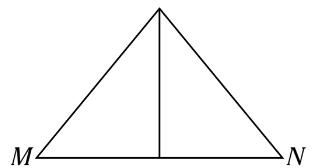
\includegraphics[width=7cm]{image/i1}\label{fig:figure2}
    \end{figure}
\end{exercise}
\\
\newpage

\begin{exercise}
    En el siguiente arreglo triangular, hallar la cantidad de puntos de contacto que se generan entre las circunferencias.
    \begin{figure}[H]
        \centering
        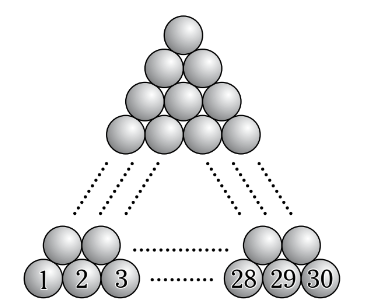
\includegraphics[width=6cm]{image/i2}\label{fig:figure3}
    \end{figure}
\end{exercise}
\\
\vspace{6cm}

\begin{exercise}
    Encontrar todos los valores $x$ tales que
    \[
        (x^2 + 2x - 7)^{(x^2 + x - 12)} = 1.
    \]
\end{exercise}